\begin{figure}[H]
	\centering
	\def\width{.1\textwidth}
	\usetikzlibrary{positioning}
	\resizebox{\textwidth}{!}{
	\begin{tikzpicture}
		\node[
			label = left:{Router}]
			(router){\includegraphics[width=\width]{images/cisco/router}};
		\node[
			below = of router, 
			label = left:{Switch}] 
			(switch){\includegraphics[width=\width]{images/cisco/workgroup_switch} };
		\node[
			below left = of switch,
			label = below:{Director}]
			(director){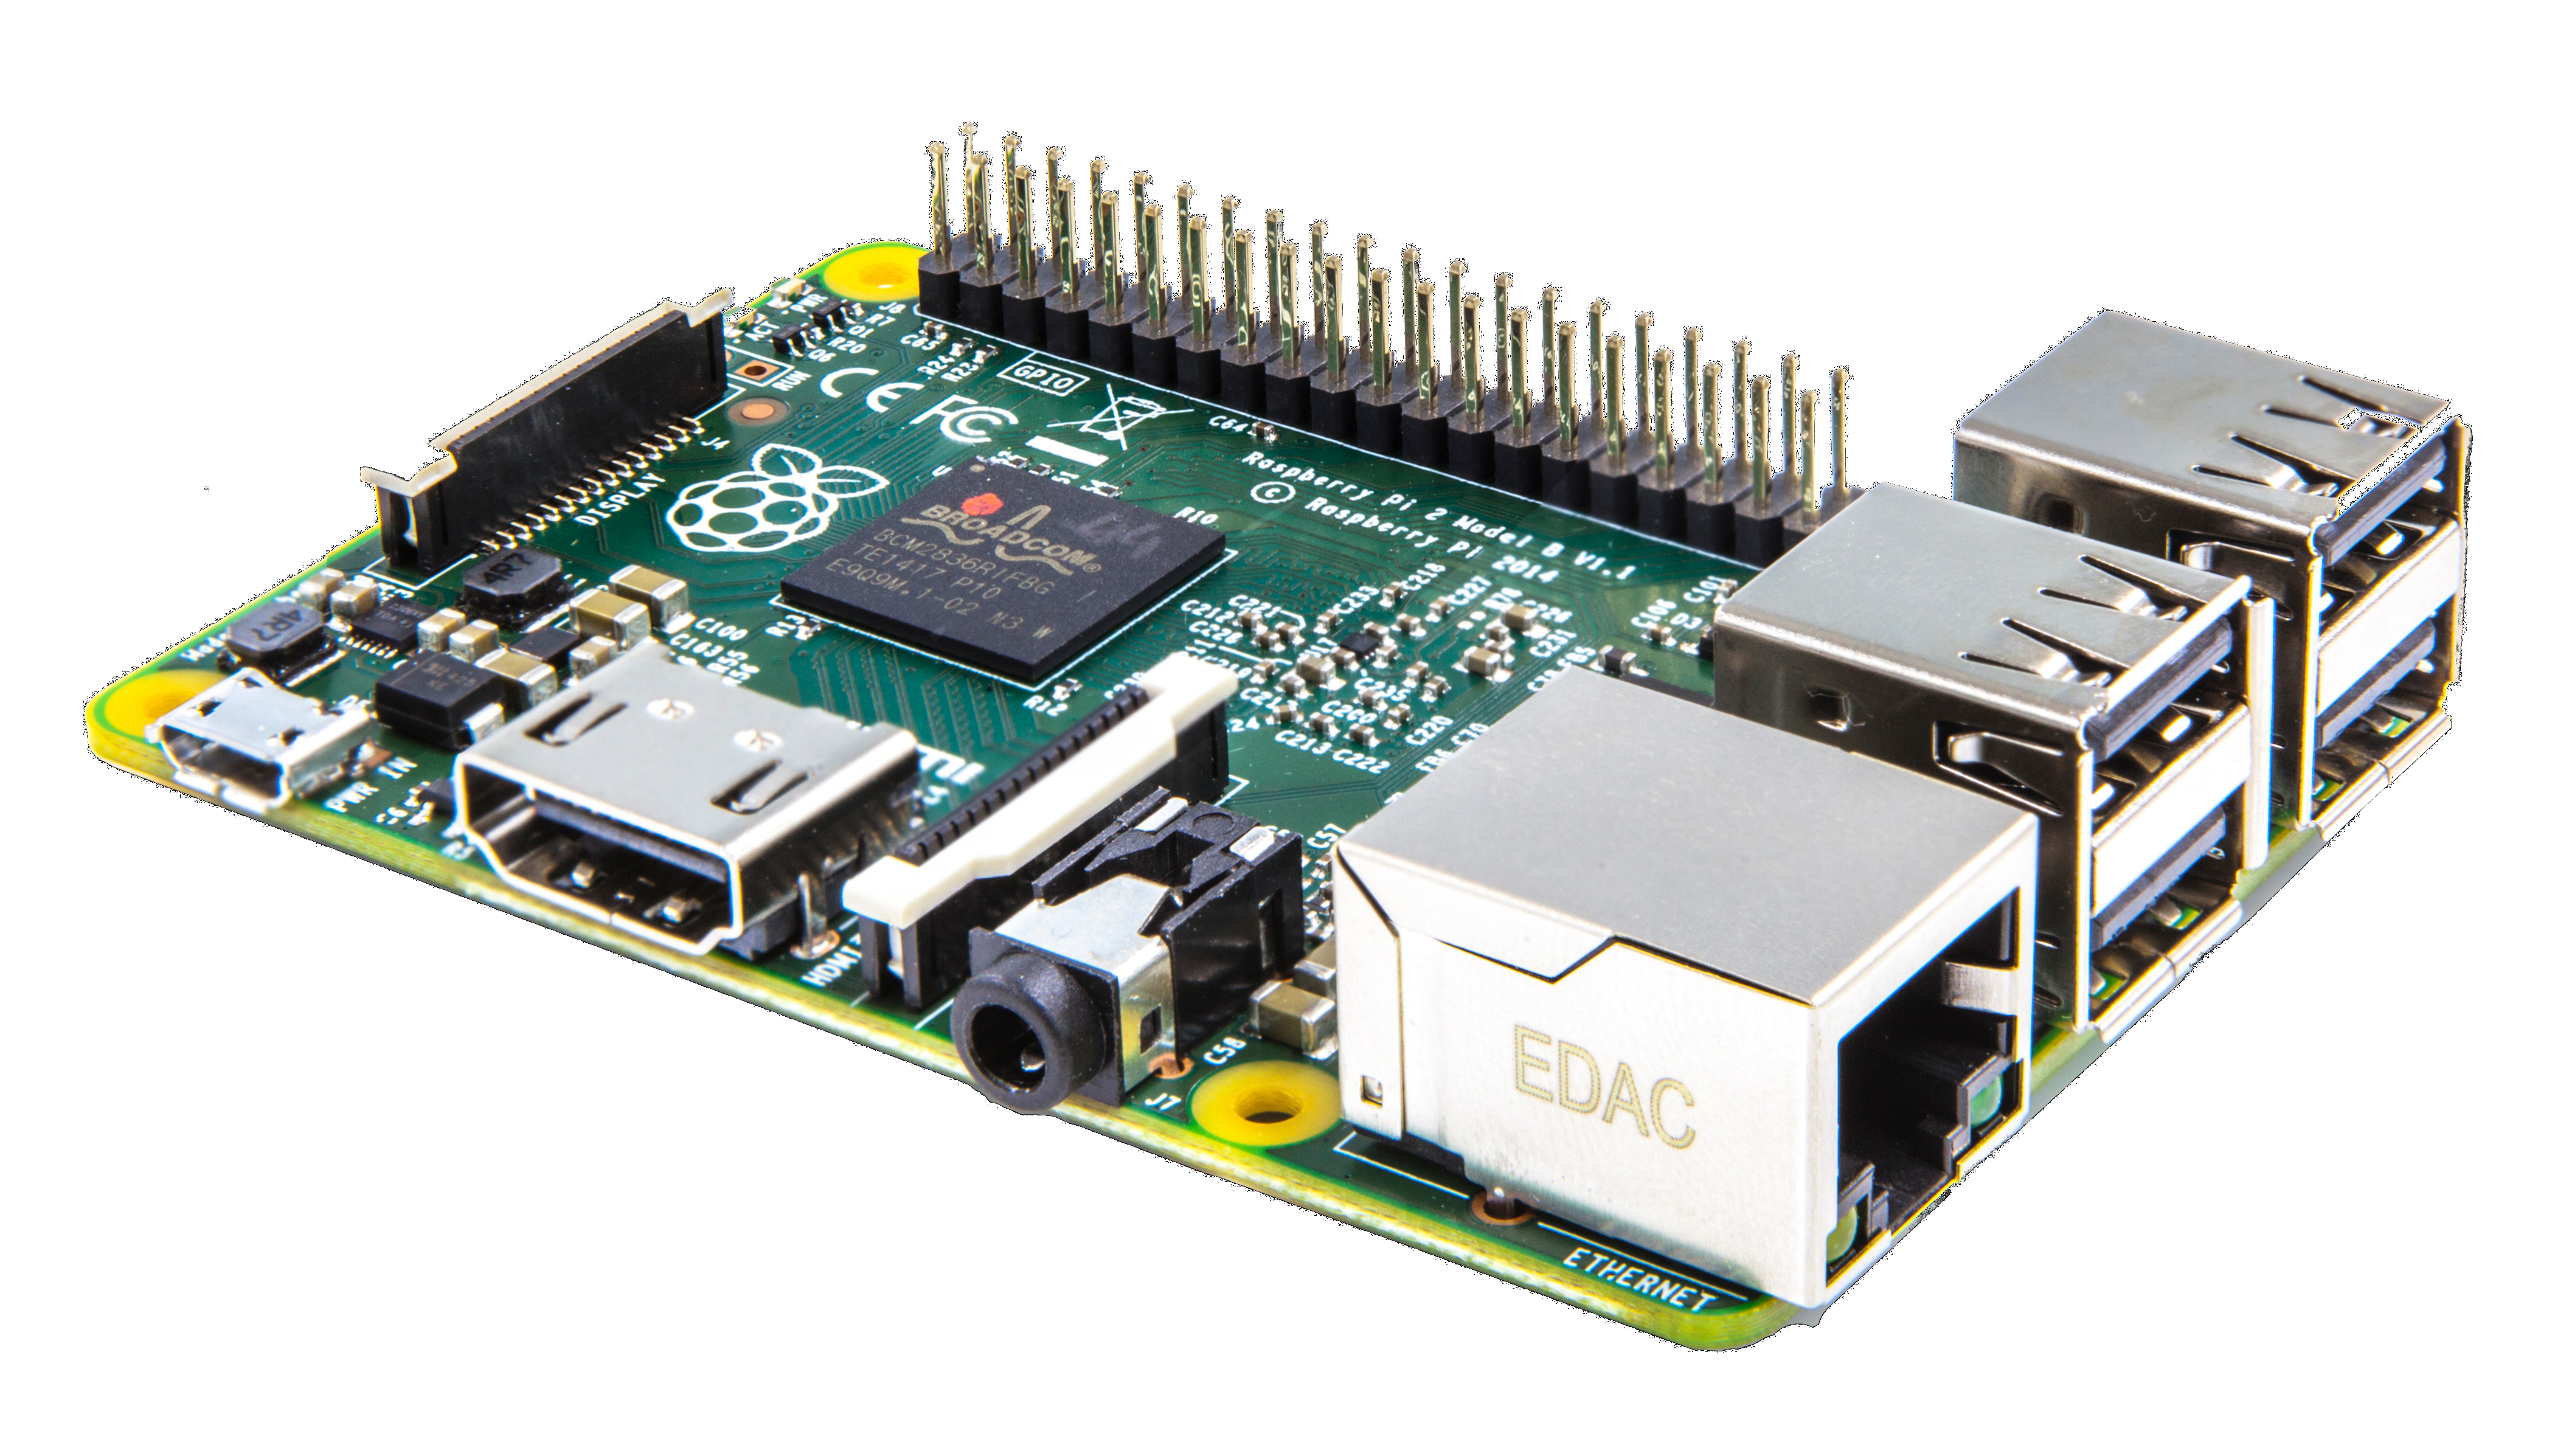
\includegraphics[width=\width]{images/raspberry}};
		\node[
			below right = of switch,
			label = below:{Músic 1}]
			(m1){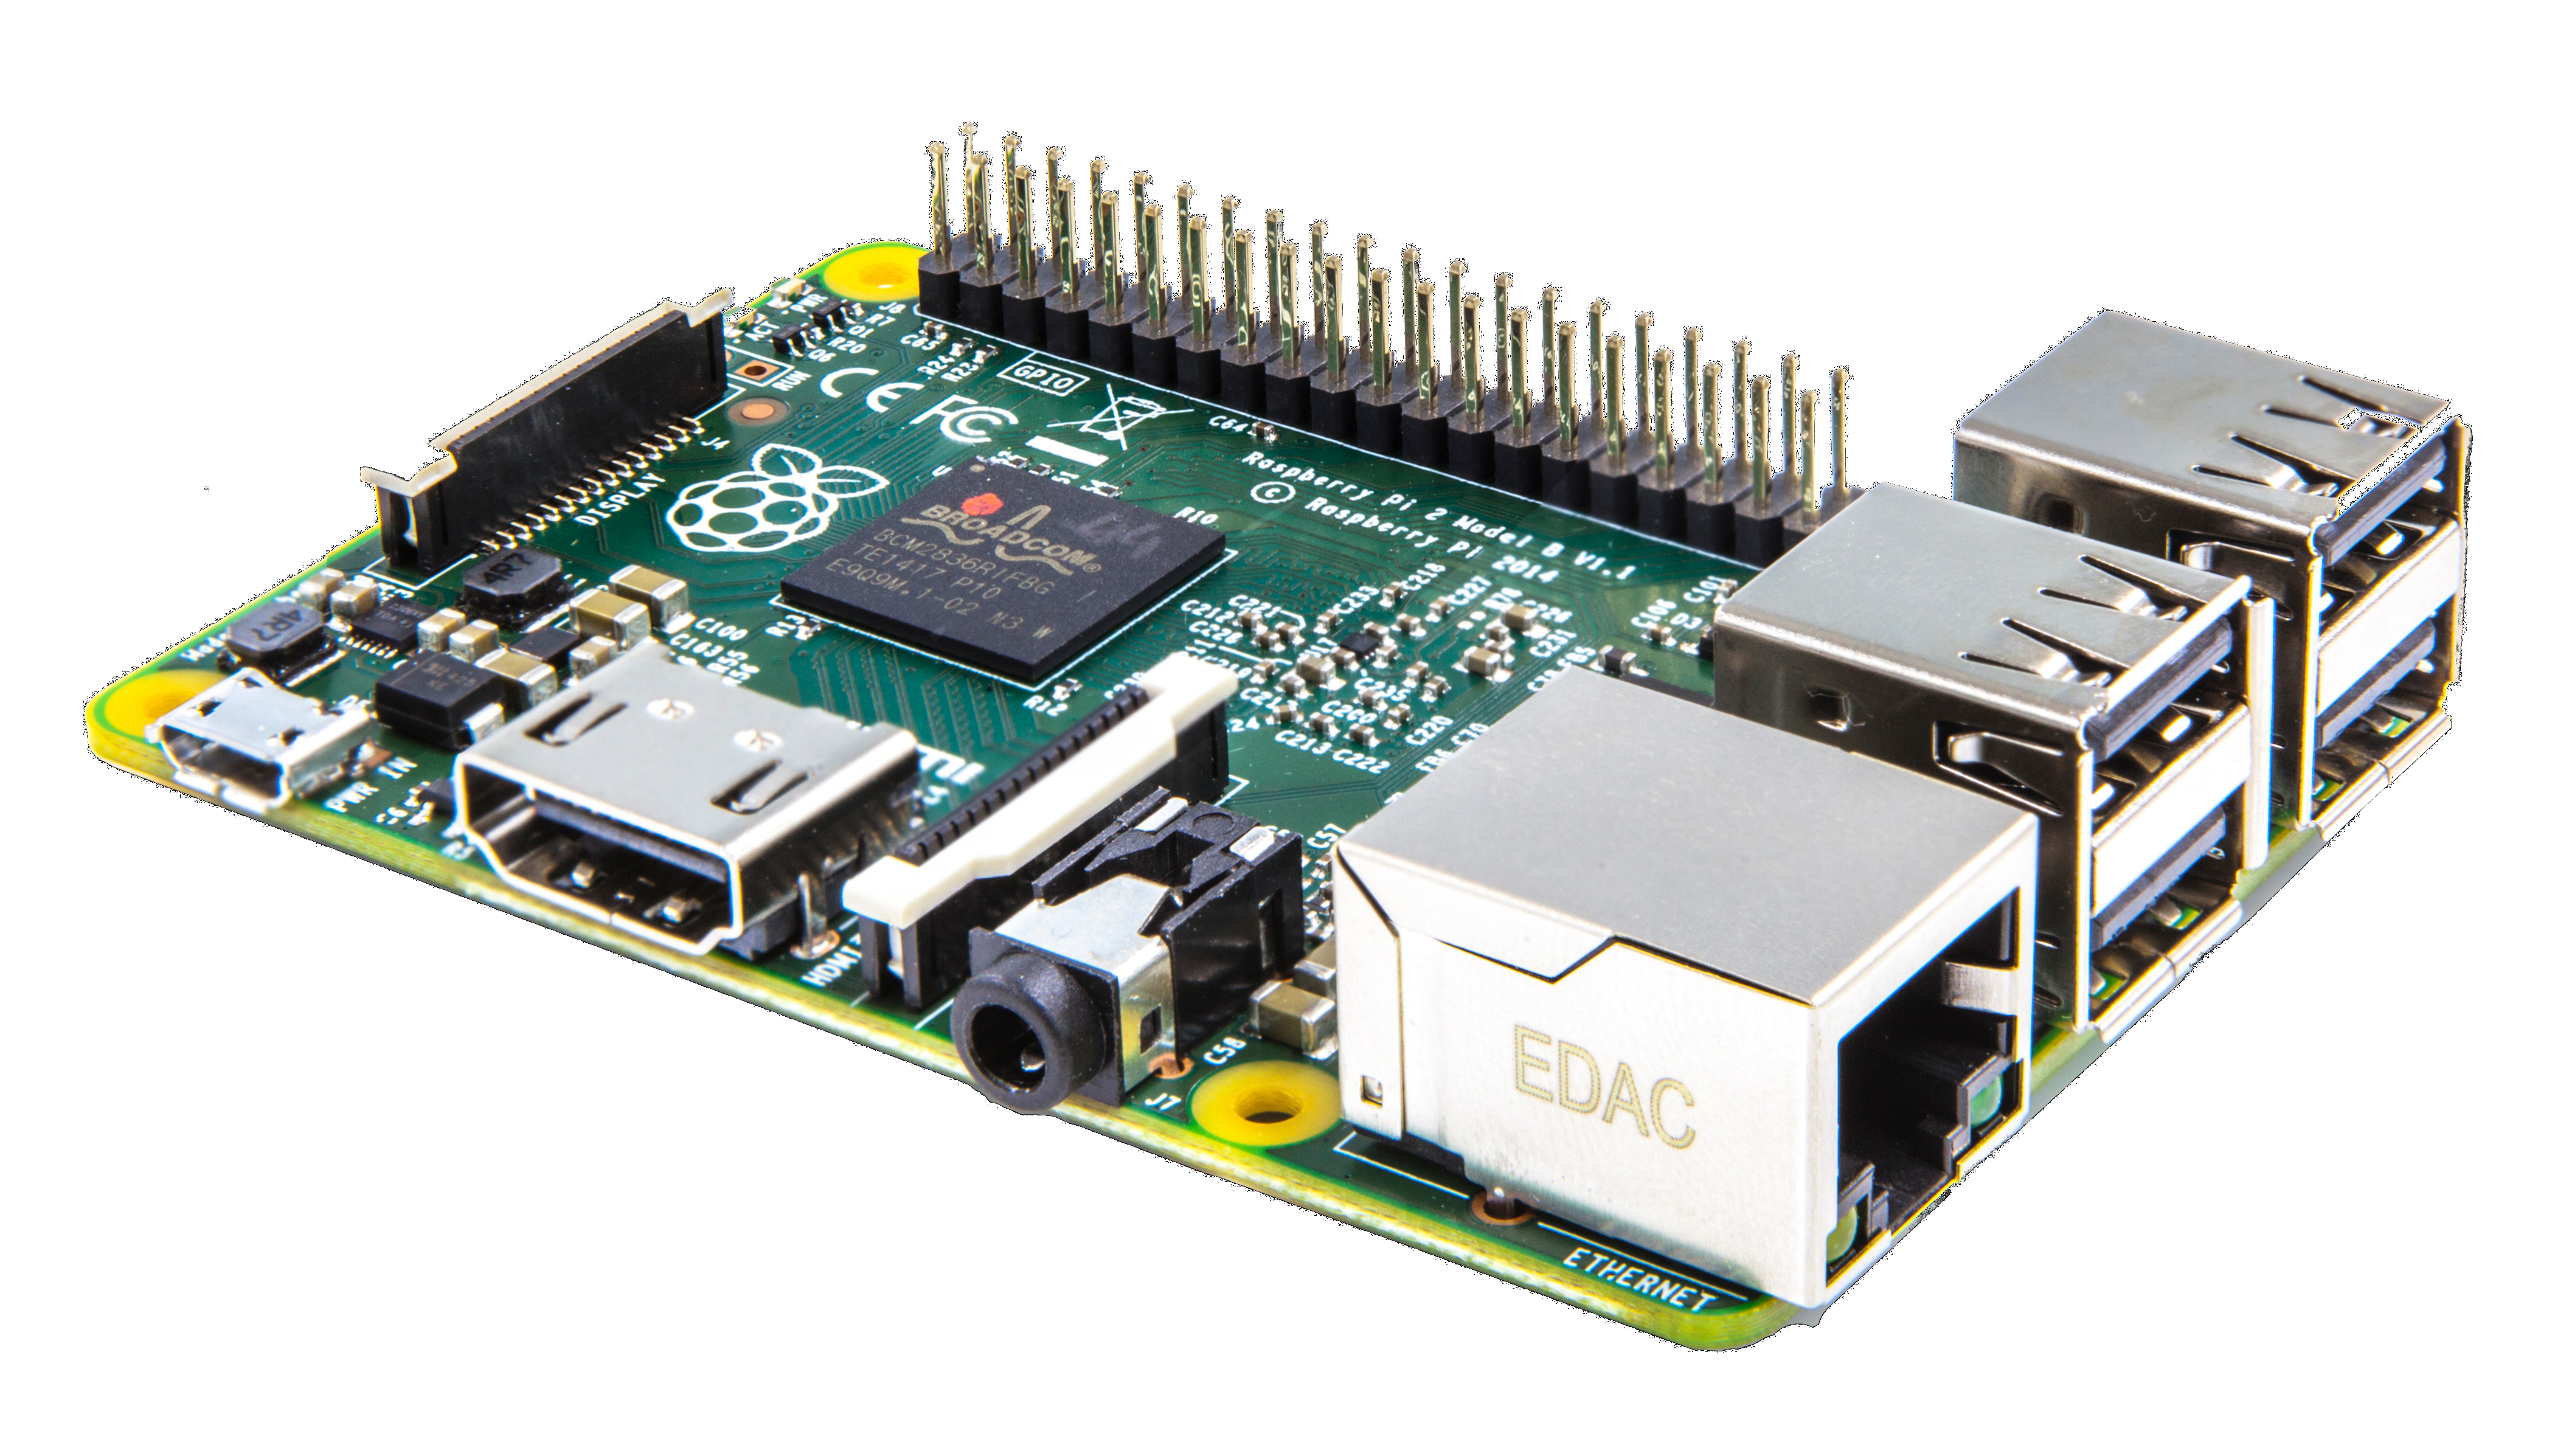
\includegraphics[width=\width]{images/raspberry}};
		\node[
			right = of m1,
			label = below:{Músic 2}]
			(m2){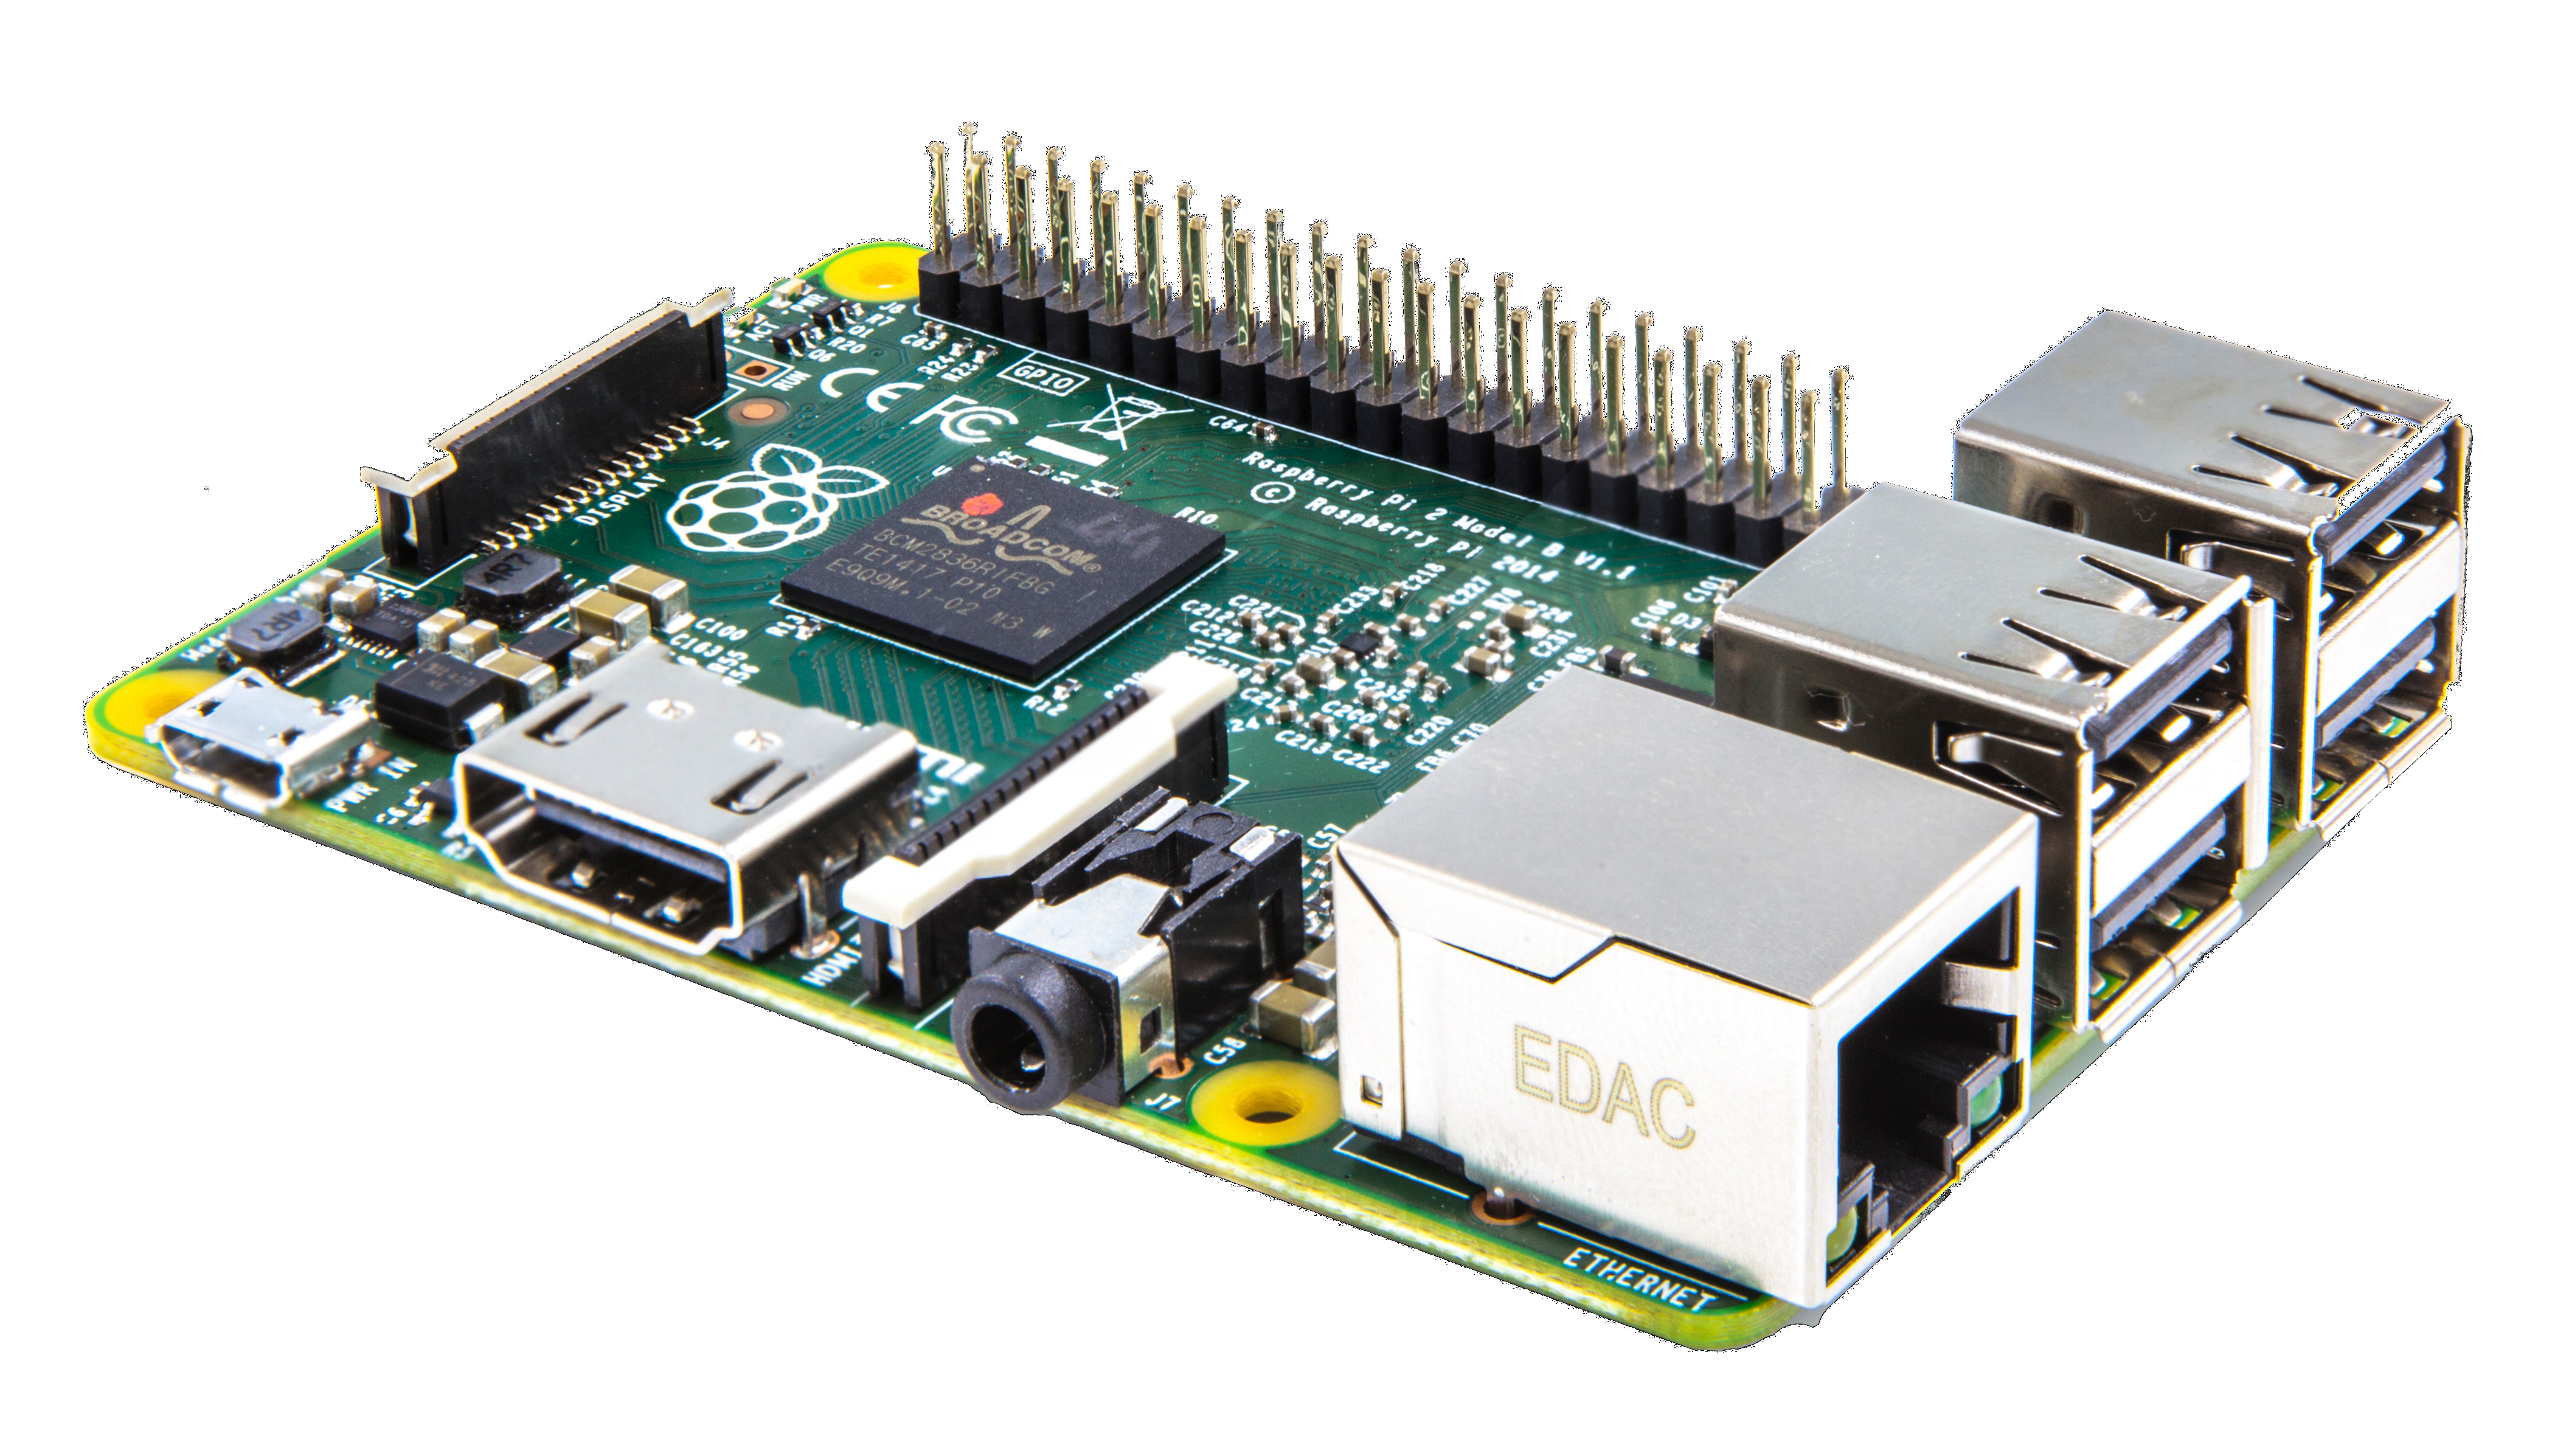
\includegraphics[width=\width]{images/raspberry}};
		\node[
			right = of m2,
			label = below:{Músic 3}]
			(m3){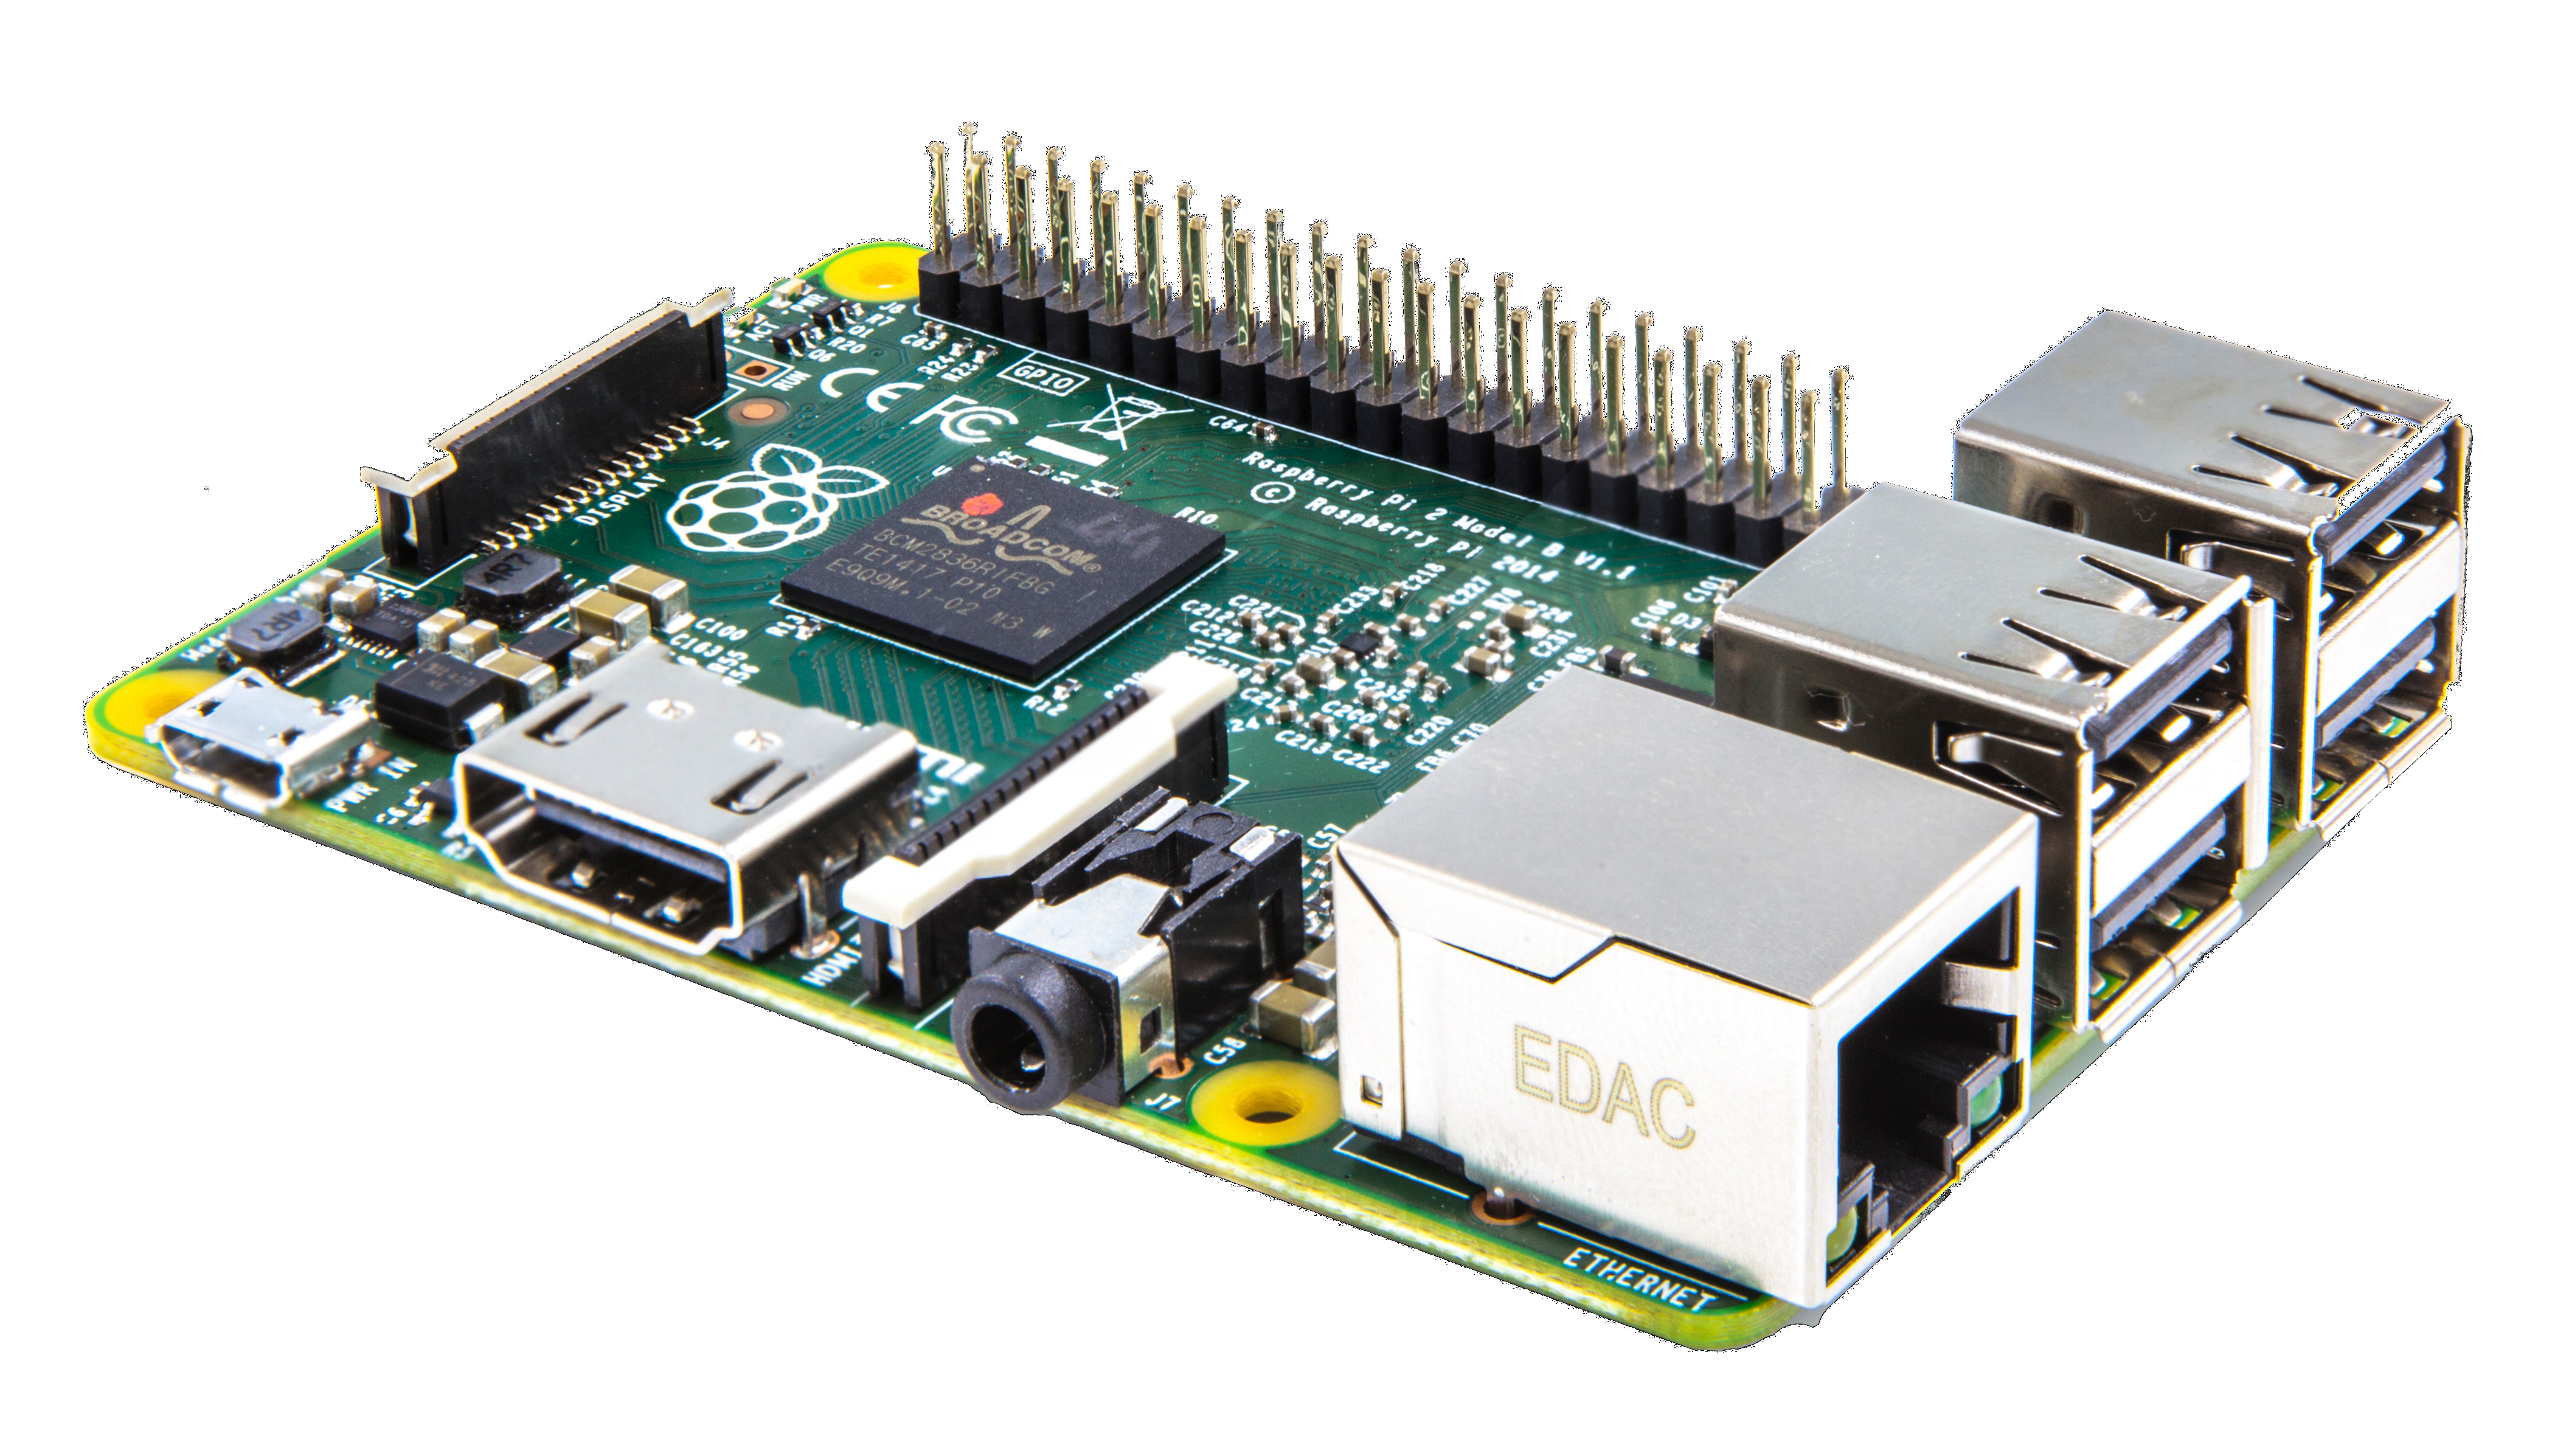
\includegraphics[width=\width]{images/raspberry}};	
		\node[
			left = of director]
			(telegram){\includegraphics[width=\width]{images/telegram}};
		
		\draw[latex-latex] (router) -- (switch);
		\draw[-latex] (director) -- (switch);
		\draw[-latex] (switch) -- (m1);
		\draw[-latex] (switch) -- (m2);
		\draw[-latex] (switch) -- (m3);
		\draw[latex-latex] (telegram) -- (director);
	\end{tikzpicture}
	}
	\caption{Esquema de funcionament de la xarxa}
\end{figure}